\chapter{\textit{User Workflow}}
Nella seguente parte del documento verrà illustrato lo ``\textit{user flow}'' per gli utenti del tipo: ``non loggato'', ``analista'' e ``sondaggista''.
\paragraph{Utenti ``non loggati''} Come possiamo osservare dalla figura \ref{fig:UserWorkflow}, gli utenti non loggati possono visualizzare la \textit{HomePage} della applicazione web, da questa possono visualizzare i dati generici della città. In alternativa alla pressione di una zona all'interno della mappa il sistema restituirà la pagina di dettaglio della zona selezionata dalla quale possono o tornare alla \textit{HomePage} o visualizzare i dettagli. Dalla \textit{HomePage} è possibile inoltre premere sul pulsante per il passaggio da ``quartieri'' a ``circoscrizioni'' e viceversa. La mappa presente nella \textit{HomePage} è interattiva e permette di spostare la visuale e di ingrandire o rimpicciolire la mappa.
\paragraph{Utenti ``loggati''} Gli utenti loggati tramite un pulsante dedicato nella \textit{HomePage} possono accedere alla pagina di \textit{login} e, inserendo le proprie credenziali, se queste sono corrette allora in base al tipo di utente questo verrà reindirizzato alla propria pagina associata. Nel caso dell'utente ``analista'' verrà reindirizzato alla HomePage con le funzionalità di analisi, mentre l'utente ``sondaggista'' verrà reindirizzato alla pagina di gestione dei sondaggi. In entrambi i casi l'utente potrà effettuare il \textit{logout} tramite un apposito menù a tendina sul quale è presente il proprio nome.
\paragraph{Utenti ``analisti''} Gli utenti di tipo ``analista'' possono visualizzare la \textit{HomePage} con le funzionalità di analisi, in particolare possono visualizzare i dati generici della città e, in alternativa alla pressione di una zona all'interno della mappa, il sistema restituirà la pagina di dettaglio della zona selezionata dalla quale possono o tornare alla \textit{HomePage} o visualizzare i dettagli. Oltre alla possibilità di cambio di visualizzazione da ``quartieri'' a ``circoscrizioni'' e viceversa, l'analista può visualizzare i dati in modalità ``tabella'' premendo sul pulsante ``mappa''/``tabella''. A differenza di tutti gli altri utenti alla pressione di una zona all'interno della mappa verrà visualizzata la pagina di dettaglio della zona selezionata per gli analisti, da questa possiamo o tornare alla \textit{HomePage} o selezionando la categoria degli attributi visualizzare i dati della zona selezionata.
\paragraph{Utenti ``sondaggista''}
Gli utenti di tipo ``sondaggista'' dalla pagina di gestione dei sondaggi possono visualizzare lo storico dei sondaggi oppure crearne uno inserendo il titolo di questo e premendo sul pulsante ``Crea un nuovo sondaggio'', è anche possibile caricare un sondaggio precedentemente creato selezionando il file e premendo sul pulsante ``Carica sondaggio''. Dalla pagina di gestione dei sondaggi è visualizzata una tabella con i sondaggi creati dall'utente, per ogni sondaggio non ancora ``completato'' è possibile continuare la compilazione premendo sopra questo, si apre dunque la pagina di gestione del sondaggio. Da questa pagina è possibile da una serie di pulsanti terminare il sondaggio e caricarlo per l'approvazione degli amministratori (col pulsante ``Termina e Carica il Sondaggio''), premere sul pulsante ``Salva ed Esci'' per salvare i cambiamenti fatti al sondaggio e tornare alla pagina dei sondaggi, oppure premere sul pulsante ``Elimina Sondaggio'' e dopo una conferma il sondaggio verrà eliminato, anche in questo caso si verrà reindirizzati alla pagina dei sondaggi. Oltre a queste azioni è possibile eseguire le azioni di voto, questo compilando i dati del cittadino che sta per votare e premendo sul pulsante ``Vota'', al termine delle operazioni si verrà reindirizzati alla pagina di gestione del sondaggio. Se sono stati commessi errori durante la compilazione del sondaggio è possibile cancellare un voto individuale.
\begin{figure}
    \centering
    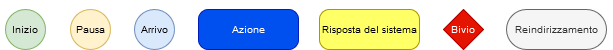
\includegraphics[width=0.9\textwidth]{User_workflow/legendeUF.png}
    \caption{User Workflow Legend}
    \label{fig:UserWorkflowLegend}
\end{figure}
\begin{figure}
    \centering
    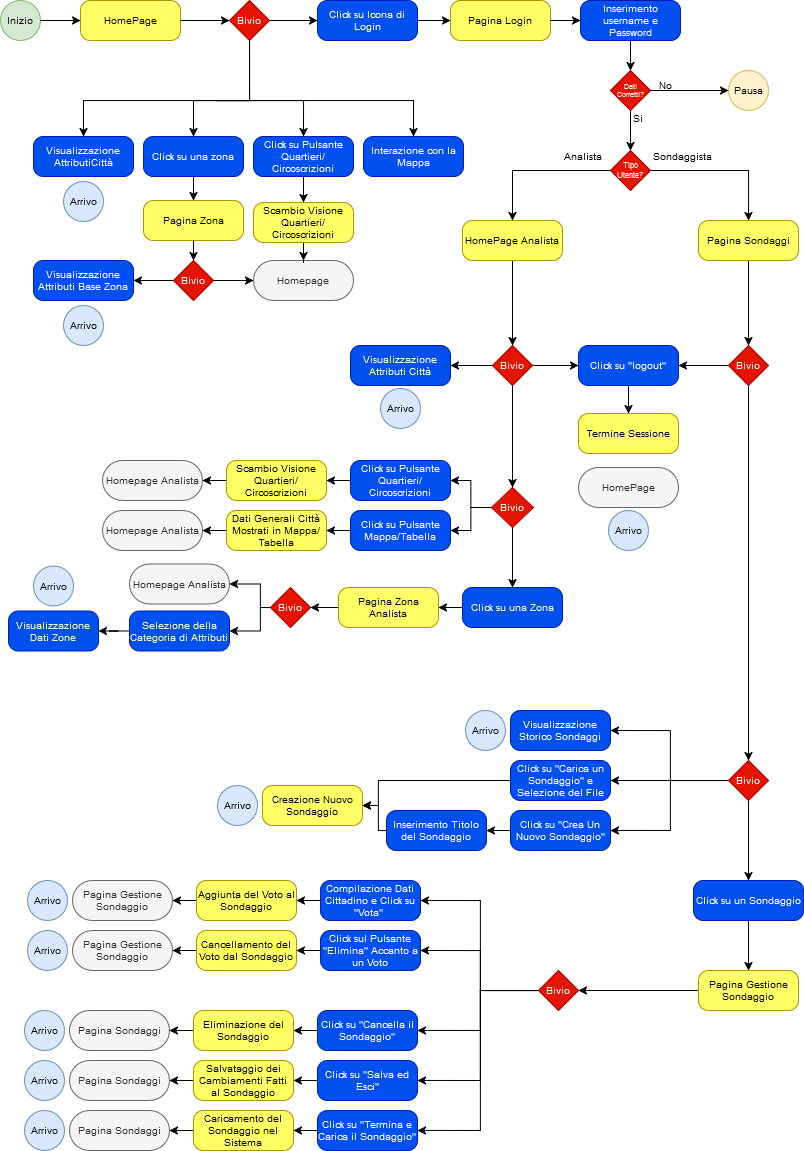
\includegraphics[width=\textwidth]{User_workflow/UserFlowComp.drawio.png}
    \caption{User Workflow}
    \label{fig:UserWorkflow}
\end{figure}